\documentclass[12pt]{article}

\usepackage{graphicx}
\usepackage[finnish]{babel}
\usepackage[utf8]{inputenc}
\usepackage{listings}

\begin{document}

\begin{titlepage}
\title{Suunnitteludokumentti}

%% {\small tietokantasovellus}

\author{Janne Ronkonen}
\maketitle
\end{titlepage}

\tableofcontents

\section{Johdanto}

\subsection{Järjestelmän tarkoitus}


Järjestelmän tarkoituksena on toimia selaimen kautta käytettävänä reseptipankkina ja ravintotietolaskurina. Järjestelmään pystytään lisäämään reseptejä joiden sisältämät ruoka-aineet merkitään ylös.

Resepteissä käytettävien ruoka-aineiden ravintoarvot voidaan syöttää joko samalla kertaa, jälkikäteen, tai käyttää jo ennestään järjestelmästä löytyviä arvoja. Näin reseptejä ja ravintoarvoja voidaan syöttää toisistaan riippumatta.

Järjestelmästä voidaan hakea reseptejä eri tavoin, esimerkiksi nimellä ja ruoka-aineiden perusteella.

Järjestelmä voi lisäksi laskea automaattisesti paljonko kutakin ravinto-ainetta reseptissä on sekä skaalata reseptejä.



\subsection{Toimintaympäristö}
Järjestelmän on tarkoitus toimia ympäristössä jossa on käytettävissä Java-ajoympäristö ja SQL-tietokanta.  
\subsection{Rajaukset}
Järjestelmään ei ole tarkoitus toteuttaa käyttäjätunnuksia, vaan kaikki käyttäjät toimivat anonyymisti. 

\subsection{Toteutusympäristö}

Työ on tarkoitus toteuttaa laitoksen palvelimella users.cs.helsinki.fi.



\section{Yleiskuva järjestelmästä}

\subsection{Sidos- ja käyttäjäryhmät}

\subsubsection{Reseptien lisääjät}

\begin{itemize}
\item lisäävät reseptejä
\item henkilöt joilla paljon reseptejä, esim. keittokirjailijat tmv?
\end{itemize}


\subsubsection{Ruoanlaittajat}
\begin{itemize}
\item etsivät reseptejä
\item täydentävät ravintoainetietoja
\end{itemize}

\subsubsection{Ravintotietofriikit}

\begin{itemize}
\item lisäävät ja täydentävät ravintoainetietoja
\end{itemize}



\subsubsection{Käyttötapaukset}
\begin{itemize}
\item Reseptin lisääminen
\item Reseptin haku nimellä tai nimen osalla
\item Reseptin haku ruoka-aineella
\item Ruoka-aineen lisääminen
\item Ruoka-aineen ravintoarvojen lisääminen
\end{itemize}




\section{Järjestelmän tietosisältö}

Järjestelmän olennaisin tietosisältö on resepti, johon liittyy tiedot siihen kuuluvista ruoka-aineista ja niiden määristä, valmistusohje sekä reseptin nimi. Ruoka-aineita voidaan lisätä myös ilman reseptin lisäämistä. 

Lisäksi järjestelmässä on tietoja ruoka-aineista, niiden sisältämistä ravintoaineista, sekä yksiköitä ja muuntokertoimia yksiköstä toiseen.



\section{Käyttöliittymän hahmotelma}

Käyttöliittymään tulee perustumaan tavanomaisille web-lomakkeille ja –sivuille. Jokaista käyttötapausta vastaa suurin piirtein yksi lomake ja yksi ”tulossivu” sekä epämääräinen joukko virhesivuja.



\appendix
\section{Tietokantakaavio}
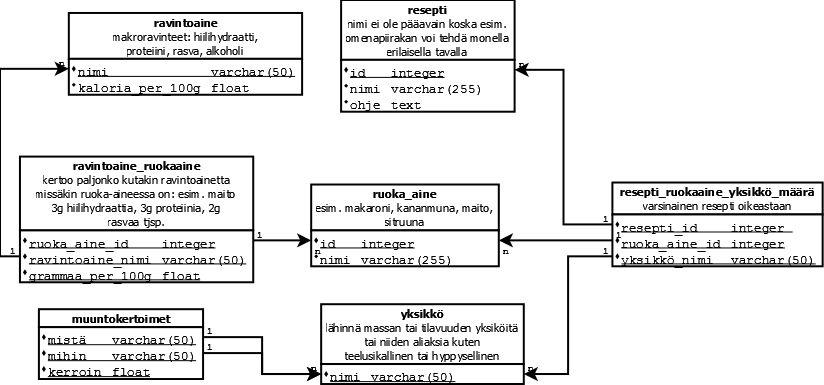
\includegraphics[width=160mm,height=100mm]{Kaavio1.png}


\appendix
\section{Create table -lauseet}
\lstinputlisting{scripts/create_tables.sql}

\end{document}
